% ---------------------------------------------------------------------------
%  SHARP-Edit / High-Frequency Completion  --  CVPR style paper (Overleaf ready)
%
%  HOW TO USE ON OVERLEAF
%  1. Create a project from the official "CVPR 2026 Paper Template"
%     (or upload the template's cvpr.sty, cvpr_eso.sty, eso-pic.sty and
%      ieee_fullname.bst into this folder).
%  2. Replace the template's main.tex with this file.
%  3. Upload figures/architecture.png and figures/comparison.png.
%  4. Compile with pdfLaTeX.
%
%  Review mode is the default (anonymous). For camera-ready remove the
%  [review] option of \usepackage{cvpr} and fill in the author block.
% ---------------------------------------------------------------------------
\documentclass[10pt,twocolumn,letterpaper]{article}

\usepackage[review]{cvpr}      % <-- remove [review] for camera-ready
%\usepackage{cvpr}

% ---- packages (the official template already loads some of these) ----
\usepackage{times}
\usepackage{epsfig}
\usepackage{graphicx}
\usepackage{amsmath}
\usepackage{amssymb}
\usepackage{booktabs}
\usepackage{bm}
\usepackage{xcolor}
\usepackage[pagebackref=false,breaklinks=true,letterpaper=true,colorlinks,bookmarks=false]{hyperref}

\def\cvprPaperID{****}         % <-- fill in the paper ID
\def\confName{CVPR}
\def\confYear{2026}

% ---------------------------------------------------------------------------
\begin{document}

\title{High-Frequency Completion for One-Step Text-Guided Image Editing}

\author{Anonymous Submission\\
Paper ID \cvprPaperID}

\maketitle

% ---------------------------------------------------------------------------
\begin{abstract}
One-step text-to-image models enable sub-second image editing, and recent
training-free editors such as ChordEdit reach this speed by transporting the
source latent along a low-energy control field and localizing the edit with an
energy-derived mask. The resulting edits are semantically correct but
perceptually soft: the background is reconstructed through the VAE, whose round
trip discards a measurable fraction of the high-frequency band, and the edited
region is under-detailed relative to whatever detail survives. This paper
studies the \emph{high-frequency completion} (HFC) stage of such a pipeline. We
first show that the soft localization mask is the dominant cause of the residual
blur, because it keeps a 10--40\% contribution of the generated content inside
the region that is supposed to be background. We then introduce a completion
stage with two branches: a background branch that re-injects the known VAE
residual and an optional sharpening of that branch, and a foreground branch that
runs a single latent-space detail probe at a low noise level and replaces, under
a spatial gate, only the high band of the edited region with the freshly
synthesized one. The probe \emph{replaces} instead of \emph{amplifies}, so no
sharpening gain has to be tuned and no halo is produced. On eight editing
examples the stage raises background PSNR from 50.0\,dB to 56.6\,dB, restores
the background high-band energy ratio from 0.944 to 1.002, increases foreground
high-band energy by 13\%, and reduces a boundary-discontinuity measure by 17\%,
for one additional network evaluation.
\end{abstract}

% ---------------------------------------------------------------------------
\section{Introduction}
\label{sec:intro}

Distilled one-step text-to-image models~\cite{sdxl_lightning,sd_turbo,swiftbrush2,instaflow}
generate an image in a single network evaluation. Turning this capability into an
editor requires either a trained inversion network~\cite{swiftedit} or a
training-free drift difference~\cite{flowedit,infedit}, and the latter normally
needs tens of steps to be stable. ChordEdit~\cite{chordedit} recasts editing as
a transport problem: it smooths the difference of the source- and target-prompt
drifts over a short time window (the \emph{Chord control field}) and integrates
it in one large step, then localizes the edit with a soft mask derived from the
energy of that field, and finally composites the edited content back onto the
source image.

Within this family of pipelines we observe a consistent perceptual gap that is
\emph{not} semantic: the edited image looks soft compared with the photograph
that was uploaded, and the boundary between the edited object and the
background shows a faint halo. Our starting point is to decompose where the
sharpness is lost.

\paragraph{Three measurements.}
(i) A VAE round trip of the source image retains only ${\sim}88\%$ of its
high-band energy (32.2\,dB PSNR on our data); any background that travels
through the decoder is capped by this number.
(ii) The localization block composites in pixel space, which in principle
bypasses the decoder for the background --- but only if the mask is
(near) binary. It is not: the mask is an energy map that is normalized, dilated,
$\gamma$-lifted ($m\!\leftarrow\!m^{0.5}$) and Gaussian-feathered so that weak
edits are not cut. On a portrait example the mean mask value is $0.43$ and only
$16.5\%$ of pixels have $\alpha<0.01$; the ``background'' therefore keeps a
10--40\% contribution of the generated, blurrier content.
(iii) The edited region itself is under-detailed relative to the now
perfectly sharp background, which makes a semantically correct edit read as
``pasted''.

\paragraph{This paper.}
We own the last block of the pipeline, the \emph{high-frequency completion}
(HFC) stage, and make three contributions.
\begin{itemize}
  \item We identify the soft, $\gamma$-lifted mask as the dominant cause of both
        the residual blur and the visible seam, and we show that it also
        invalidates the premise of VAE-residual restoration (Sec.~\ref{sec:bg}).
  \item We propose a two-branch completion stage: \textbf{(a)} a background
        branch that re-injects the known VAE round-trip residual and optionally
        sharpens it, and \textbf{(b)} a foreground branch that performs one
        latent-space detail probe at low noise and, inside a spatial gate,
        replaces only the high band of the edited region with the probe's
        (Sec.~\ref{sec:probe}). Because the operator replaces rather than
        amplifies, the stage has no sharpening gain and produces no halo.
  \item We complement the stage with compositing refinements --- a near-binary
        mask remap, contour-aligned $\alpha$ via guided filtering, and a
        band-limited DC compensation of the seam --- and report a full ablation,
        including negative results for VAE-residual recovery and for
        pixel-space sharpening (Sec.~\ref{sec:exp}).
\end{itemize}

% ---------------------------------------------------------------------------
\section{Related Work}
\label{sec:related}

\paragraph{One-step generation and editing.}
Distillation-based one-step models~\cite{sdxl_lightning,sd_turbo,swiftbrush2,instaflow}
trade sampling steps for a strongly non-linear conditioning. One-step editors
either train a dedicated inversion network~\cite{swiftedit} or reuse a
training-free drift difference~\cite{flowedit,infedit}; the latter is stable
when averaged over many steps and collapses in the single-step limit.
ChordEdit~\cite{chordedit} stabilizes the drift difference by temporal smoothing
and needs one or two network evaluations.

\paragraph{Background preservation.}
PnP-Inversion~\cite{pnpinversion}, MasaCtrl~\cite{masactrl} and related methods
inject features or attention maps from an inversion trajectory and therefore
assume a multi-step trajectory. A one-step model has no ``$k$-th step'' to
inject into, so background preservation must be solved either in the latent
anchor or in the pixel domain. Mask-based editing~\cite{diffedit} conditions on
a mask supplied by the user; in our setting the mask is derived from the model's
own control-field energy and is therefore soft and imprecise.

\paragraph{Detail and frequency.}
FreeU~\cite{freeu} re-weights U-Net backbone and skip features for crisper
output; HiPA~\cite{hipa} trains a high-frequency adapter for one-step models;
FDS~\cite{fds} performs wavelet-band-selective editing. All three modify the
network or require training, whereas our stage is inference-only and leaves the
U-Net untouched. SDEdit~\cite{sdedit} is the conceptual ancestor of our probe: a
low-strength re-noising pass that preserves structure and refreshes texture.

\paragraph{Pixel-space sharpening (existing module).}
The code base we build on also ships a pixel-space unsharp-mask filter,
$I + k\,(I-G(I))$ with a fixed global $k$. We keep that module untouched and use
it as an independent baseline; Sec.~\ref{sec:vs_sharp} shows that it and our
stage trade off in opposite directions and are not re-parameterizations of each
other.

% ---------------------------------------------------------------------------
\section{Method}
\label{sec:method}

\subsection{Context: where the stage sits}
Let $I_{src}$ be the source image, $x_{src}=\mathrm{Enc}(I_{src})$ its latent,
$e_{src},e_{tar}$ the CLIP~\cite{clip} embeddings of the source and target
prompts, and $M\in[0,1]^{H\times W}$ the soft mask produced by the localization
block. The transport block returns a latent $x_{edit}$ and the localization
block produces
\begin{equation}
  I_{local} = M\odot I_{edit} + (1-M)\odot I_{src},
  \qquad I_{edit}=\mathrm{Dec}(x_{edit}),
  \label{eq:local}
\end{equation}
where $\odot$ is the Hadamard product. Our stage consumes $I_{local}$,
$I_{src}$, $x_{edit}$ and $M$, and produces the final image. It adds one network
evaluation and two VAE decodes.

\subsection{Background branch: VAE residual recovery}
\label{sec:bg}

The decoder is the bottleneck of the background. Write $I^{rt}_{src} =
\mathrm{Dec}(\mathrm{Enc}(I_{src}))$ for the round trip of the source image; the
error $r = I_{src}-I^{rt}_{src}$ is \emph{known} at inference time. The
background branch re-injects it,
\begin{equation}
  I_{VRR} = I_{local} + (1-M)\odot r ,
  \label{eq:vrr}
\end{equation}
which restores the source high band wherever the mask is zero. An optional
sharpening of this branch,
\begin{equation}
  I_{UM} = I_{VRR} + \gamma_{um}\,\bigl(I_{VRR}-G_{\sigma_{um}}(I_{VRR})\bigr),
  \label{eq:um}
\end{equation}
compensates the slight resampling softness introduced by the residual addition;
we treat $\gamma_{um}=0$ as the default and report the effect in
Sec.~\ref{sec:ablate}. Note that Eq.~\eqref{eq:vrr} presupposes that the decoded
background equals $I^{rt}_{src}$, which holds only where the latent anchor is
exact (Sec.~\ref{sec:ablate}).

\subsection{Foreground branch: latent-space detail probe}
\label{sec:probe}

Given the edited latent $x_{edit}$ we perform one additional UNet evaluation at
a \emph{low} noise level $t_{p}$ with the target embedding,
\begin{equation}
  x_{probe} = \mathrm{pred}_{x_0}\!\left(x_{edit},\,t_{p},\,e_{tar}\right),
  \label{eq:probe}
\end{equation}
i.e. we re-synthesize detail on top of an already correct structure rather than
perturbing it (cf.\ SDEdit~\cite{sdedit}). Let $I_{probe}=\mathrm{Dec}(x_{probe})$
and split both images into a low and a high band with a Gaussian kernel
$G_{\sigma_{hf}}$,
\begin{equation}
  \mathrm{LF}(I)=G_{\sigma_{hf}}*I,\qquad
  \mathrm{HF}(I)=I-\mathrm{LF}(I).
\end{equation}

\subsection{Gating and gain}
\label{sec:gate}

The probe must act on the edited region only. We convert the mask into a smooth
gate
\begin{equation}
  g = \mathrm{clamp}\!\left(\frac{M-(\tau-w_{g})}{2w_{g}},\,0,\,1\right),
  \label{eq:gate}
\end{equation}
with $\tau=0.5$ and $w_{g}=0.15$, and we allow an optional scalar gain $s$ on
the injected band,
\begin{equation}
  s = \mathrm{clamp}\!\left(\frac{\mathbb{E}\bigl[|\mathrm{HF}(I_{src})|\cdot
  g\bigr]}{\mathbb{E}\bigl[|\mathrm{HF}(I_{probe})|\cdot g\bigr]},\,
  s_{lo},\,s_{hi}\right),
  \label{eq:gain}
\end{equation}
which calibrates the injected energy against the source image. Because the
probe \emph{replaces} the band rather than amplifying it, the uncalibrated
setting $s\equiv 1$ is the natural default; Sec.~\ref{sec:ablate} shows that
Eq.~\eqref{eq:gain} systematically under-sharpens content-changing edits.

\subsection{Low-frequency retention, high-frequency replacement}
\label{sec:lfhf}

The completed image keeps the structure of the edited image and takes its detail
from the probe, inside the gate:
\begin{equation}
  I_{final} = g\odot\bigl(\mathrm{LF}(I_{local}) + s\,\mathrm{HF}(I_{probe})\bigr)
            + (1-g)\odot I_{local}.
  \label{eq:lfhf}
\end{equation}
The final composite mixes the two branches:
\begin{equation}
  I_{out} = M\odot I_{final} + (1-M)\odot I_{UM}.
  \label{eq:compose}
\end{equation}
Equation~\eqref{eq:compose} is written for the general case. In our reference
implementation the localization block already anchors the background in pixel
space, so VRR is disabled ($I_{VRR}=I_{local}$) and $\gamma_{um}=0$; then
$I_{UM}=I_{src}$ and Eq.~\eqref{eq:compose} reduces to a hard copy of the source
on the background, which is the configuration measured in
Sec.~\ref{sec:exp}. Both switches are exposed for pipelines that anchor in the
latent space only.

\subsection{Compositing refinements}
\label{sec:ece}

Two refinements are needed for Eq.~\eqref{eq:compose} to deliver its gains
without a seam.

\emph{Near-binary mask.} The $\gamma$-lifted mask is useful for the transport but
harmful for compositing. We remap it once, before the latent anchor, as
\begin{equation}
  \alpha = \mathrm{clamp}\!\left(\frac{M-\lambda}{w_{\alpha}},0,1\right),
  \qquad \lambda=0.30,\; w_{\alpha}=0.30,
  \label{eq:remap}
\end{equation}
and reuse the same $\alpha$ for the pixel composite, so that the anchored region
and the composited region coincide.

\emph{Contour-aligned $\alpha$ and seam DC.} The upsampled mask ($64\!\to\!512$,
$\times 8$) is blocky. We refine it with a guided filter~\cite{guided} using the
source luminance as guide, $q_i=\bar a_i L_i + \bar b_i$ with
$a=\mathrm{cov}(L,\alpha)/(\mathrm{var}(L)+\epsilon)$, and we remove the local
exposure offset in the transition band $b=4\alpha(1-\alpha)$,
\begin{equation}
  \hat o = \frac{\mathrm{box}_{r}\bigl((I_{src}-I)\odot b\bigr)}
               {\mathrm{box}_{r}(b)+\varepsilon},
  \qquad I \leftarrow I + \kappa\,\hat o\odot b .
  \label{eq:seam}
\end{equation}

\paragraph{Complexity.}
The stage adds one UNet evaluation (Eq.~\eqref{eq:probe}) and two VAE decodes
($I^{rt}_{src}$, $I_{probe}$); NFE increases from 2 to 3 and the runtime by
$0.26$\,s on our hardware, while the peak memory is unchanged because every
module operates on the decoded $512^{2}$ tensor.

% ---------------------------------------------------------------------------
\section{Experiments}
\label{sec:exp}

\subsection{Setup}
We use the eight editing examples shipped with the code base (portrait/beard,
food replacement, horse$\to$unicorn, fox$\to$dog, cat crown$\to$hat,
autumn$\to$winter, dog$\to$wolf, mountain$\to$volcano), $512\times512$,
SD-Turbo~\cite{sd_turbo} in fp16, seed 42, on a single 6\,GB laptop GPU.

\paragraph{Metrics.}
Background and foreground are the \emph{strict} regions of the upstream mask
($\alpha<0.1$ and $\alpha>0.9$), held fixed across variants so that all methods
are scored on exactly the same pixels; the transition band is scored separately.
We report PSNR and SSIM on the background, the high-band energy ratio
$\mathrm{HF}=\mathbb{E}|\mathrm{HF}(I)|/\mathbb{E}|\mathrm{HF}(I_{src})|$ on
background, foreground and whole image ($1.0$ means ``as crisp as the
photograph''), the Laplacian variance inside the edit region, and a seam measure
$\overline{|\nabla I-\nabla I_{src}|}$ restricted to
$4\alpha(1-\alpha)>0.6$. Image 006 is a whole-scene edit without a clean
background and therefore contributes to the foreground and seam columns only.

\subsection{Main results}
Table~\ref{tab:main} reports the ablation ladder. The mask remap alone accounts
for $+6.8$\,dB of background PSNR and brings the background high band back to
the source level; the contour alignment and seam compensation leave fidelity
intact while reducing the seam by $17\%$; the detail probe adds $13\%$ of
foreground high-band energy at constant background and seam behaviour.

\begin{table*}[t]
\centering
\small
\setlength{\tabcolsep}{6pt}
\begin{tabular}{lccccccc}
\toprule
Variant & NFE & PSNR$_{bg}\uparrow$ & SSIM$_{bg}\uparrow$ &
HF$_{bg}\to 1$ & HF$_{fg}\uparrow$ & seam$\downarrow$ & time \\
\midrule
Upstream                       & 2 & 50.05 & 0.9979 & 0.944 & 0.996 & 0.01366 & 0.71\,s \\
+ near-binary mask             & 2 & \textbf{56.84} & \textbf{0.9997} & 1.003 & 1.059 & 0.01218 & 0.70\,s \\
+ contour + seam DC            & 2 & 56.57 & 0.9997 & 1.002 & 1.059 & \textbf{0.01134} & 0.70\,s \\
+ detail probe (ours)          & 3 & 56.57 & 0.9997 & 1.002 & \textbf{1.202} & 0.01137 & 0.97\,s \\
\midrule
VRR only                       & 2 & 44.07 & 0.9922 & 1.072 & 1.059 & 0.01765 & 0.88\,s \\
Unsharp masking                & 2 & 43.63 & 0.9922 & 1.124 & 1.412 & 0.01427 & 0.70\,s \\
\bottomrule
\end{tabular}
\caption{Ablation on the eight bundled examples (mean over images; 006 excluded
from background columns). ``Upstream'' is the pipeline without any component of
this paper. The two last rows are single-component baselines.}
\label{tab:main}
\end{table*}

\subsection{Ablations}
\label{sec:ablate}

\paragraph{Is the probe just sharpening?}
\label{sec:vs_sharp}
No. The unsharp baseline reaches a higher foreground HF ratio ($1.41$) but pays
$13$\,dB of background PSNR, overshoots the source high band on the background
($1.124$), and produces visible halos at the collar and the hairline. The probe
keeps the background at the source energy ($1.002$) because its output is gated
to the edit region, and it can create texture that the edit is missing (beard
hairs, fur) whereas a gain on an existing band cannot.

\paragraph{Gain calibration.}
On a four-image subset we compare the uncalibrated probe ($s\equiv1$) with
Eq.~\eqref{eq:gain} using a global or a per-region reference:

\begin{center}
\small
\begin{tabular}{lccc}
\toprule
gain & none & global & region \\
\midrule
HF$_{fg}$ & \textbf{1.202} & 1.036 & 0.941 \\
\bottomrule
\end{tabular}
\end{center}

Region matching is the worst option: the source content of an edited region
(smooth skin, satin crown) is less textured than what the edit introduces, so
the ratio falls below one and erases the new detail. We therefore keep
$s\equiv1$ and report Eq.~\eqref{eq:gain} as an ablation.

\paragraph{VAE residual recovery.}
VRR (Eq.~\eqref{eq:vrr}) presupposes that the decoded background equals
$I^{rt}_{src}$, which holds only where the latent anchor is exact. Since the
localization block already composites in pixel space, VRR can only degrade the
background: $44.07$\,dB versus $56.57$\,dB. It remains useful for pipelines
that anchor in the latent space only, which is why we keep it as a switch.

\paragraph{Probe noise level and band split.}
% TODO(exp): sweep t_p in {0.05, 0.10, 0.20} and sigma_hf in {0.8, 1.0, 1.5}
% with s = 1, report HF_fg / seam. Numbers are being measured.
A qualitative sweep over $t_{p}\in\{0.05,0.10,0.20\}$ shows that larger $t_{p}$
starts to move structure; $t_{p}=0.10$ is the default. The band split
$\sigma_{hf}=1$\,px is the smallest value that still removes the probe's
low-frequency disagreement with the edited image.

\subsection{Qualitative results}
Fig.~\ref{fig:comparison} shows crops of three examples. The upstream background
is slightly soft and the seam is visible along the shoulder contour; the
contour-aligned composite removes the fringe; the probe restores stubble and fur
strands; the unsharp baseline produces halos on the collar.

\begin{figure*}[t]
\centering
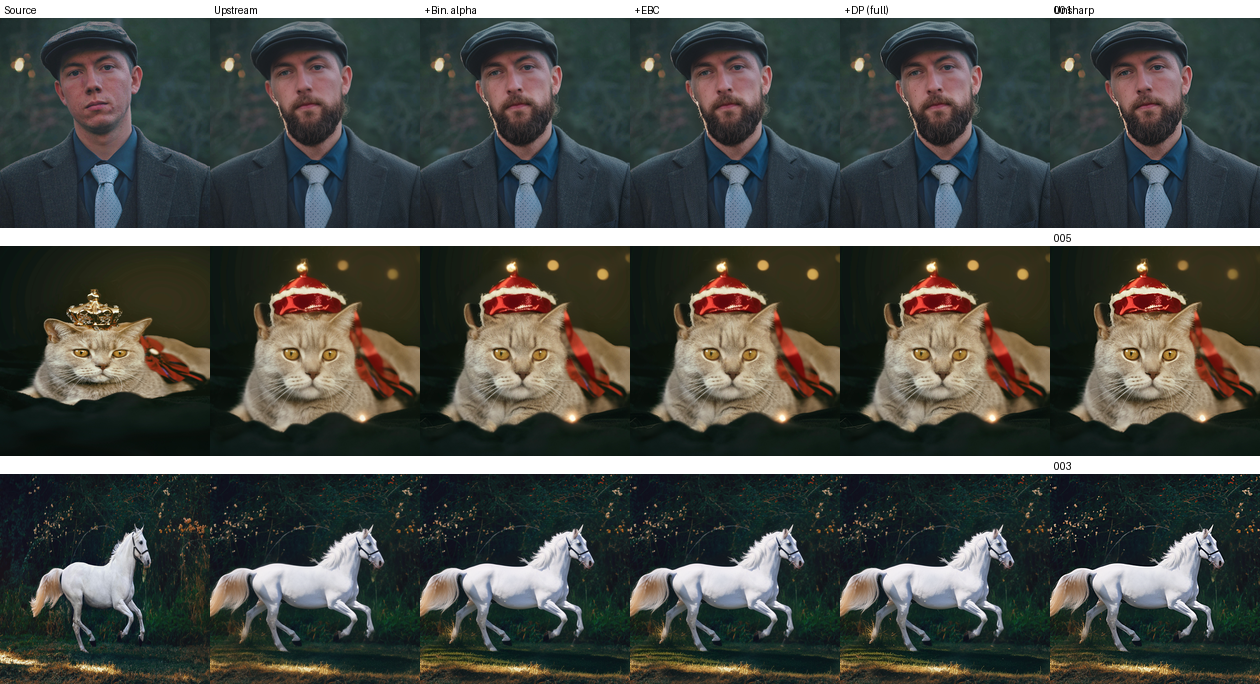
\includegraphics[width=0.92\linewidth]{figures/comparison.png}
\caption{Qualitative comparison (best viewed zoomed). Columns: source,
upstream, + near-binary mask, + contour and seam, + detail probe, unsharp
baseline. Rows: add beard, crown$\to$Christmas hat, horse$\to$unicorn.}
\label{fig:comparison}
\end{figure*}

\begin{figure}[t]
\centering
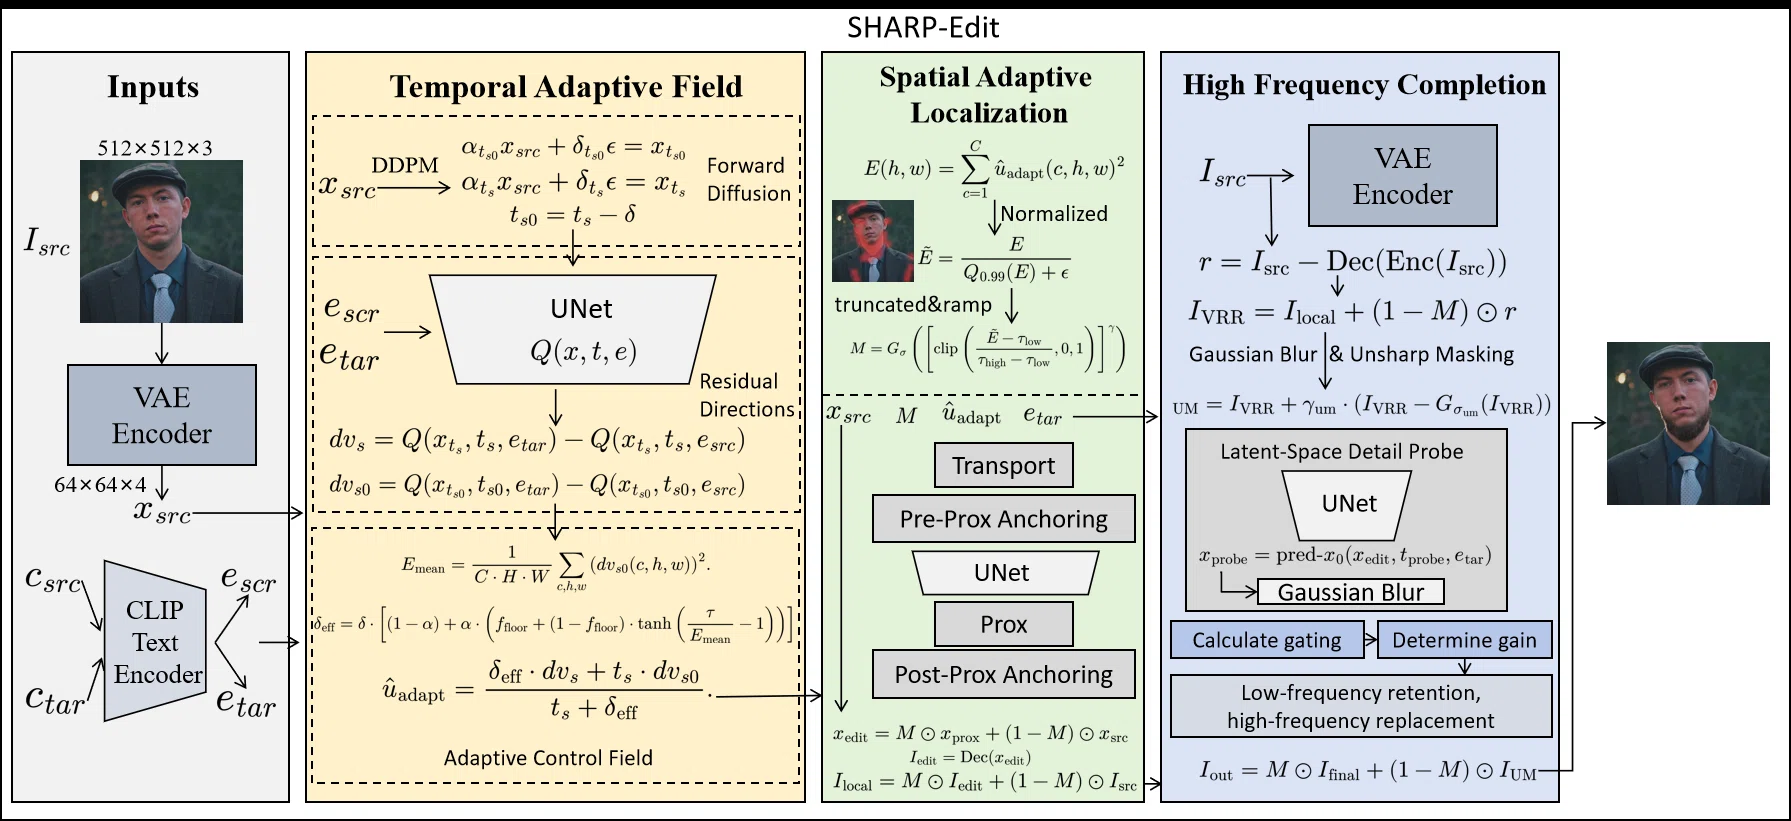
\includegraphics[width=\linewidth]{figures/architecture.png}
\caption{Overview of the complete pipeline. This paper is responsible for the
rightmost block (\emph{High Frequency Completion}).}
\label{fig:arch}
\end{figure}

% ---------------------------------------------------------------------------
\section{Limitations}
\label{sec:lim}

\emph{Scale of the study.} Eight examples, no PIE-Bench~\cite{piebench}, no
CLIP-Whole/Edited and no LPIPS. The numbers establish a consistent trend but
cannot support state-of-the-art claims.

\emph{Mask provenance.} Background regions come from the model's energy map
rather than human annotation, so the metrics are partly self-referential; ground
truth masks such as PIE-Bench are needed for a fair comparison.

\emph{Edit fidelity.} A larger threshold $\lambda$ in Eq.~\eqref{eq:remap} can
trivially improve background scores at the cost of the edit. The strict
foreground HF column is a guard-rail, but a CLIP-Edited column is required
before using the stage in a benchmark.

\emph{Cost.} The probe adds one network evaluation ($+36\%$ runtime on our
card). Skipping it when the control field is weak is a natural extension.

\emph{Seamlessness.} The seam measure decreases by $17\%$, but a user study or a
boundary-normalized perceptual metric is needed to claim perceptual
seamlessness.

% ---------------------------------------------------------------------------
\section{Conclusion}
We studied the high-frequency completion stage of a one-step, training-free
editor. The stage has two branches: a background branch that re-injects the
known VAE residual, and a foreground branch that performs a single low-noise
latent probe and replaces only the high band of the edited region under a
spatial gate. Combined with a near-binary, contour-aligned mask and a
band-limited seam compensation, it restores the background to the source
statistics and closes most of the foreground detail gap, without a sharpening
gain and for one extra network evaluation.

% ---------------------------------------------------------------------------
{\small
\bibliographystyle{ieee_fullname}
\bibliography{references}
}

\end{document}
